% Chapter X

\chapter{Infection through the lense of genomics} % Chapter title

\label{ch:01-02} % For referencing the chapter elsewhere, use \autoref{ch:name} 

%----------------------------------------------------------------------------------------

The toolset to detect and investigate bacterial infection traditionally included biochemical assays and microscopy. The recent technological advances in DNA sequencing have spurred a rapid extension of this toolset with NGS-derived methods. Here we introduce the different ways genomics can provide biological insights into the biology of bacterial pathogens.

\section{Pathogen characterization}

The most fundamental task related to infection in biomedical research is to detect the presence of infectious agents and characterize them. This allows to test patients presenting suspicious symptoms for the presence of known pathogens, or determine the pathogenicity of a particular strain. 

Genotyping was traditionally achieved using molecular biology techniques, such as \acrfull{RFLP} or \acrfull{PFGE} \cite{ochoa-diazBacterialGenotypingMethods2018}. These techniques rely on the negative charge of the DNA molecules. When put in a gel submitted to an electromagnetic field, these molecules will migrate along the electrical current. The migration distance is proportional to the size of molecules. After migration is complete, the gel can be treated with chemical markers to highlight the location of DNA molecules. This will reveal discrete bands of similar-length DNA fragments. Together these bands form a bar-code which can be interpreted by the scientist to draw conclusion about the number and size of these fragments. In the case of \acrshort{RFLP}, the genome is prealably digested by \Gls{restriction enzyme}s. The digestion will result in a series of fragments whose lengths can be seen on the gel. Bacterial genotypes wil have different mutations which will affect the digestion pattern and resulting barcode on the gel.

While these methods work well to determine differences between alleles, they do not inform us on the actual DNA sequence involved. The advent of DNA sequencing made it possible to directly link phenotype with associated sequences of nucleotides. \acrfull{WGS} provides accurate information on an organism's genotype, down to down to the \acrfull{SNP}, allowing to define genotypes at a finer scale. The main shortcoming of \acrshort{WGS} is its higher cost than other genotyping techniques, but the recent plummeting of sequencing costs have made it releatively affordable. These advantages have made \acrshort{WGS} a popular approach in clinical settings.

\section{Genomics to probe homeostasis}

When host cells are exposed to or infected by a pathogen, their homeostatic state is disrupted. This disruption is a combination of alterations caused by the pathogen to colonize the host cell and host-triggered immune reactions to improve its survival. These two components can usually be unentangled in infection experiments by using a disabled pathogen. The pathogen will still harbour the antigens triggering host reactions, but will be unable to cause any harms. One can then deduce the pathogen-caused disruptions by comparing the infection results from a standard and disabled pathogen. 

Multiple levels of regulation are affected upon infection, from signalling to epigenetic modifications \cite{rolandoLegionellaPneumophilaType2014}, and over the years, a vast arsenal of NGS techniques have been developed to read these regulatory states. 

The most frequently used feature is gene expression. The transcribed RNAs present in the sample can be reverse-transcribed into cDNA and sequenced and the relative abundance of each gene's transcript allows to quantify the expression of the whole genome, known as the transcriptome. Transcriptomes can then be compared between different conditions to find out which genes undergo perturbations during infection. 

Many levels of regulation allow to fine tune gene expression in eukaryote (Fig. \ref{fig:01-02:transcriptional-regulation}). Regulatory elements can be directly encoded by the sequence and trigger the recruitment of protein complexes to fine tune gene expression. Epigenetic changes, in the form of chemical modification of histone proteins offer yet another way to regulate gene expression in eukaryotes. The amount of these epigenetic marks can be measured along the genome using another NGS-derived technique known as \acrfull{ChIPseq}. In \acrshort{ChIPseq}, the chromatin sample is crosslinked with formaldehyde to generate covalent bonds between proteins and DNA. The sample is then sonicated to break the DNA into smaller fragments. Beads coated with specific antibodies against a protein of interest (e.g. an epigenetic mark) are then added and the beads are then precipitated to retrieve them. The crosslinked is then reversed and the DNA fragments purified. This allows to retrieve all genomic regions that were bound to the protein of interest. 

\begin{figure}
    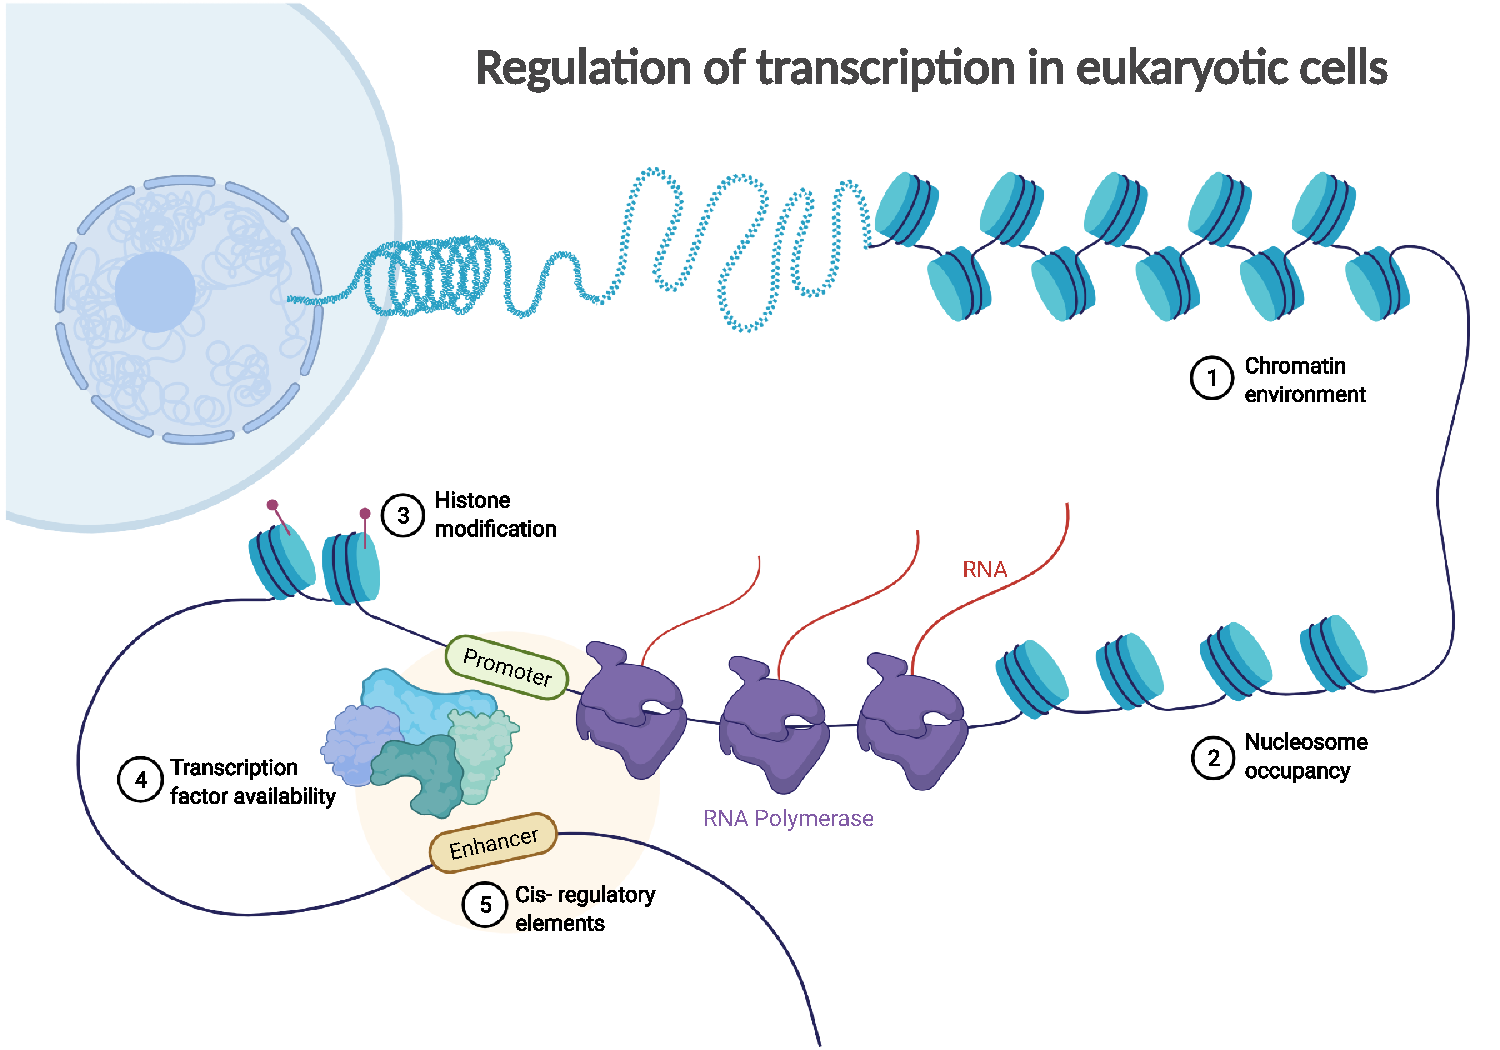
\includegraphics[width=\textwidth]{Parts/Part01/gfx/transcriptional_regulation_levels.pdf}
    \caption{Regulation of transcription in eukaryotic cells. Visual summary of the different levels at which transcription can be regulated. At the largest scale (1), the chromatin environment can form structures affecting transcription. The open space between nucleosome can also affect accessibility of protein complexes to gene sequences (2). Chemical modifications on histone proteins form an epigenetic code defining the recruitment of transcriptional complexes on the genome (3). The availablity of those factors (4) and the proximity of regulatory sequences such as enhancers (5) provide another level of transciptional regulation. Reprinted from “Regulation of Transcription in Eukaryotic Cells”, by BioRender.com (2020). Retrieved from https://app.biorender.com/biorender-templates }
    \label{fig:01-02:transcriptional-regulation}
\end{figure}


\section{Capturing chromosome conformation}

Although DNA is a linear (or circular) molecule, it can fold back on itself and form three-dimensional structures which have several benefits compared to a linear structure. These benefit include compactness: For example, the human chromosome 1 consists of 250 millions nucleotides each spaced by 0.34nm \cite {langridgeMolecularConfigurationDeoxyribonucleic1960}. If straightened, the chromosome would be 85mm long, but the whole genome fits in a nucleus where the diameter is around 10$\mu m$. Another key feature of genome folding is the regulation of gene expression through higher order structures. Compacting large regions of the genome by spreading of \Gls{heterochromatin} allows to downregulate their activity. Smaller scale structures allow to fine tune gene regulation more locally. For example, \Gls{chromatin} loops can bring enhancer and promoters in close spatial proximity even if they would otherwise be far apart on the linear sequence. Compact chromatin domain also form local neighbourhoods where different loci are in close spatial proximity, while loci in distinct domains are isolated from each other. All these levels of spatial regulation are important to understand the coordination of the gene expression programme with other celluar processes.

\subsection{3C technologies}

The use of genomics to investigate the three-dimensional organisation of the genome started with the invention of \acrfull{3C} \cite{dekkerCapturingChromosomeConformation2002}. This technique allowed to measure the frequency of physical interactions a pair of loci (Fig. \ref{fig:01-02:3c}). This is done by crosslinking the genome with formaldehyde, which forms stable bonds between DNA and proteins, and subsequently digesting the genome with a restriction enzyme. Genomic regions closer in space will be crosslinked together more frequently, resulting in pairs or complexes of chromatin fragments from different genomic regions that were spatially interacting. The digested genome is then religated. Loci which are closer in space are religated more often with each other in the population of cells. The crosslink is then reverted and primers from two regions of interest are added to perform qPCR. This allows to measure the quantity of religated products containing the two loci of interest. Thus, 3C allows to quantify the spatial proximity between two known genomic loci.

\begin{figure}[htb]
    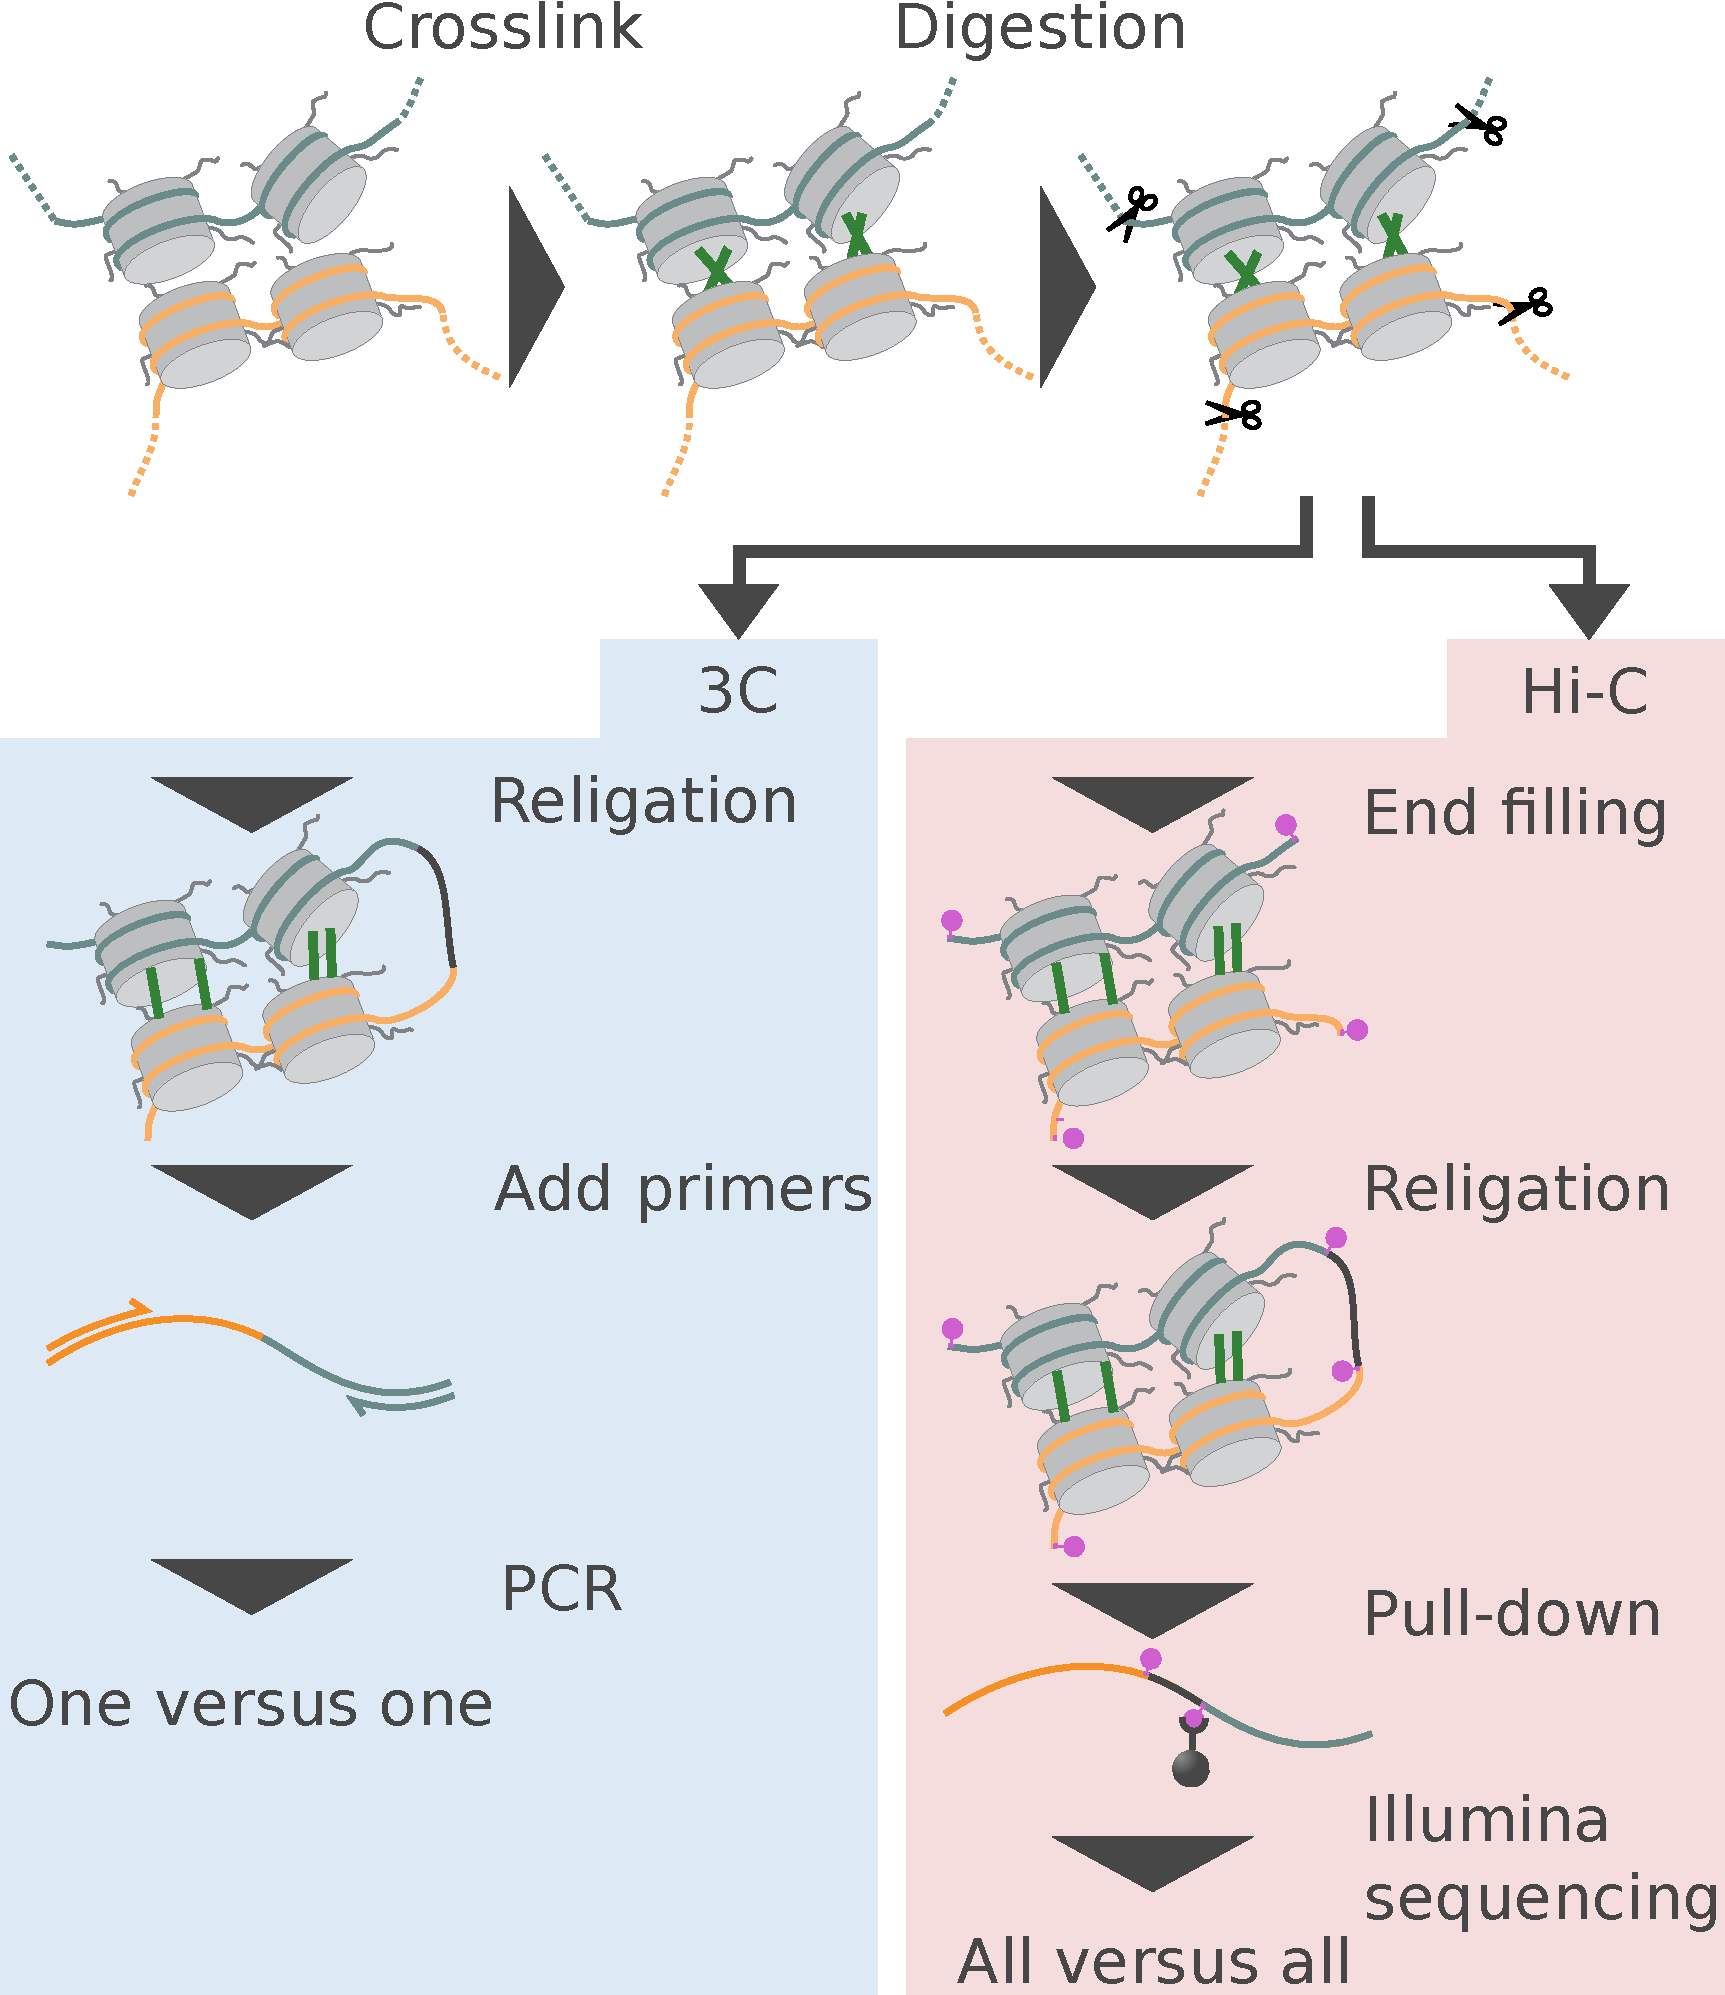
\includegraphics[width=\textwidth]{Parts/Part01/gfx/3c_protocol.pdf}
    \caption{Chromosome conformation capture protocol: Chromosome conformation capture protocol share common steps (top): The chromatin is first crosslinked to form covalent DNA-protein bonds and then digested using a restriction enzyme. The Hi-C protocol subsequently differs from the original 3C protocol. In 3C (left), fragments are religated, the crosslinked is reversed and specific primers are added to amplify a pair of known loci. This allows to quantify interaction between 2 loci. In Hi-C (right), the fragments ends are filled with biotinylated nucleotides (pink), religated and the crosslinked is reversed. Streptavidin beads are then used to pull down religation products which are then sequenced.}
	\label{fig:01-02:3c}
\end{figure}

Since then, many derivatives of the \acrshort{3C} technique have been developed. The most significant improvement was brought by Hi-C (Fig. \ref{fig:01-02:3c}, right). This method shares several steps with 3C, the main difference being that next generation sequencing is used instead of qPCR. This allows to quantify the interaction frequency of all versus all loci in the genome instead of using specific primers for a pair of locus. In Hi-C, fragment ends are filled with biotin prior to religation \cite{lieberman-aidenComprehensiveMappingLongRange2009}. The religation products are then pulled-down using streptavidin beads (which have high affinity for biotin), which allows to specifically retain digested  and religated products for sequencing.

The information generated by Hi-C experiments is a list of contacts between all pairs of restriction fragments in the genome. These contacts are most commonly visualized using contact maps (Fig. \ref{fig:01-02:hic}a), which are two entry tables represented as color-coded matrices. The color of each value in the matrix is proportional to its value and reflects the interaction frequency between the associated pair of fragments. Those contact maps are an indirect representation of the tri-dimensional folding of chromosomes and are rich in information.

The various folding structures formed by chromatin are created by DNA binding proteins. The most common example is the \acrfull{CTCF}, a transcription factor that also acts as an "architectural protein" structuring chromatin. Molecular motors such as cohesin and other \acrfull{SMC} family proteins slide along DNA to operate various roles. When cohesin is loaded onto the chromosome, it can extrude two strands of DNA in opposite directions through it's ring-shaped structure, a process known as loop extrusion \cite{fudenbergFormationChromosomalDomains2016}. When cohesin encounters a roadblock protein such as \acrshort{CTCF} the extrusion stops, forming a chromatin loop and maintaining contact between the two DNA strands. Depending on the location of those roadblocks, this can form stable interactions between distant genomic regions. 

Each spatial structure formed by chromatin is reflected on the contact map as a distinct pattern (Fig. \ref{fig:01-02:hic}b). At the largest scale, chromosomes are isolated from each other in the nucleus, occupying distinct "chromosome territories". This is reflected as dark squares along the diagonal of the whole genome contact map as each chromosome interacts more with itself than any other chromosome (Fig. \ref{fig:01-02:hic}a). Within each chromosome chromatin forms "insulation domains", known as \acrfull{TAD}s in mammals. Genes sharing the same domain are in close proximity, while being isolated from genes in neighbouring domains . Genes within the same domain also tend to be co-regulated \cite{noraSpatialPartitioningRegulatory2012}. Domains form dark squares along the diagonal of a chromosome, due to the enriched intra-domain interactions at the expense of inter-domain contacts (Fig. \ref{fig:01-02:hic}b, bottom). At a finer scale, chromatin loops are visible on contact maps as dots away from the diagonal (Fig. \ref{fig:01-02:hic}b, middle). The coordinates of those dots correspond to the genomic positions of roadblocks which stopped the extrusion process.

\begin{figure}[htb]
    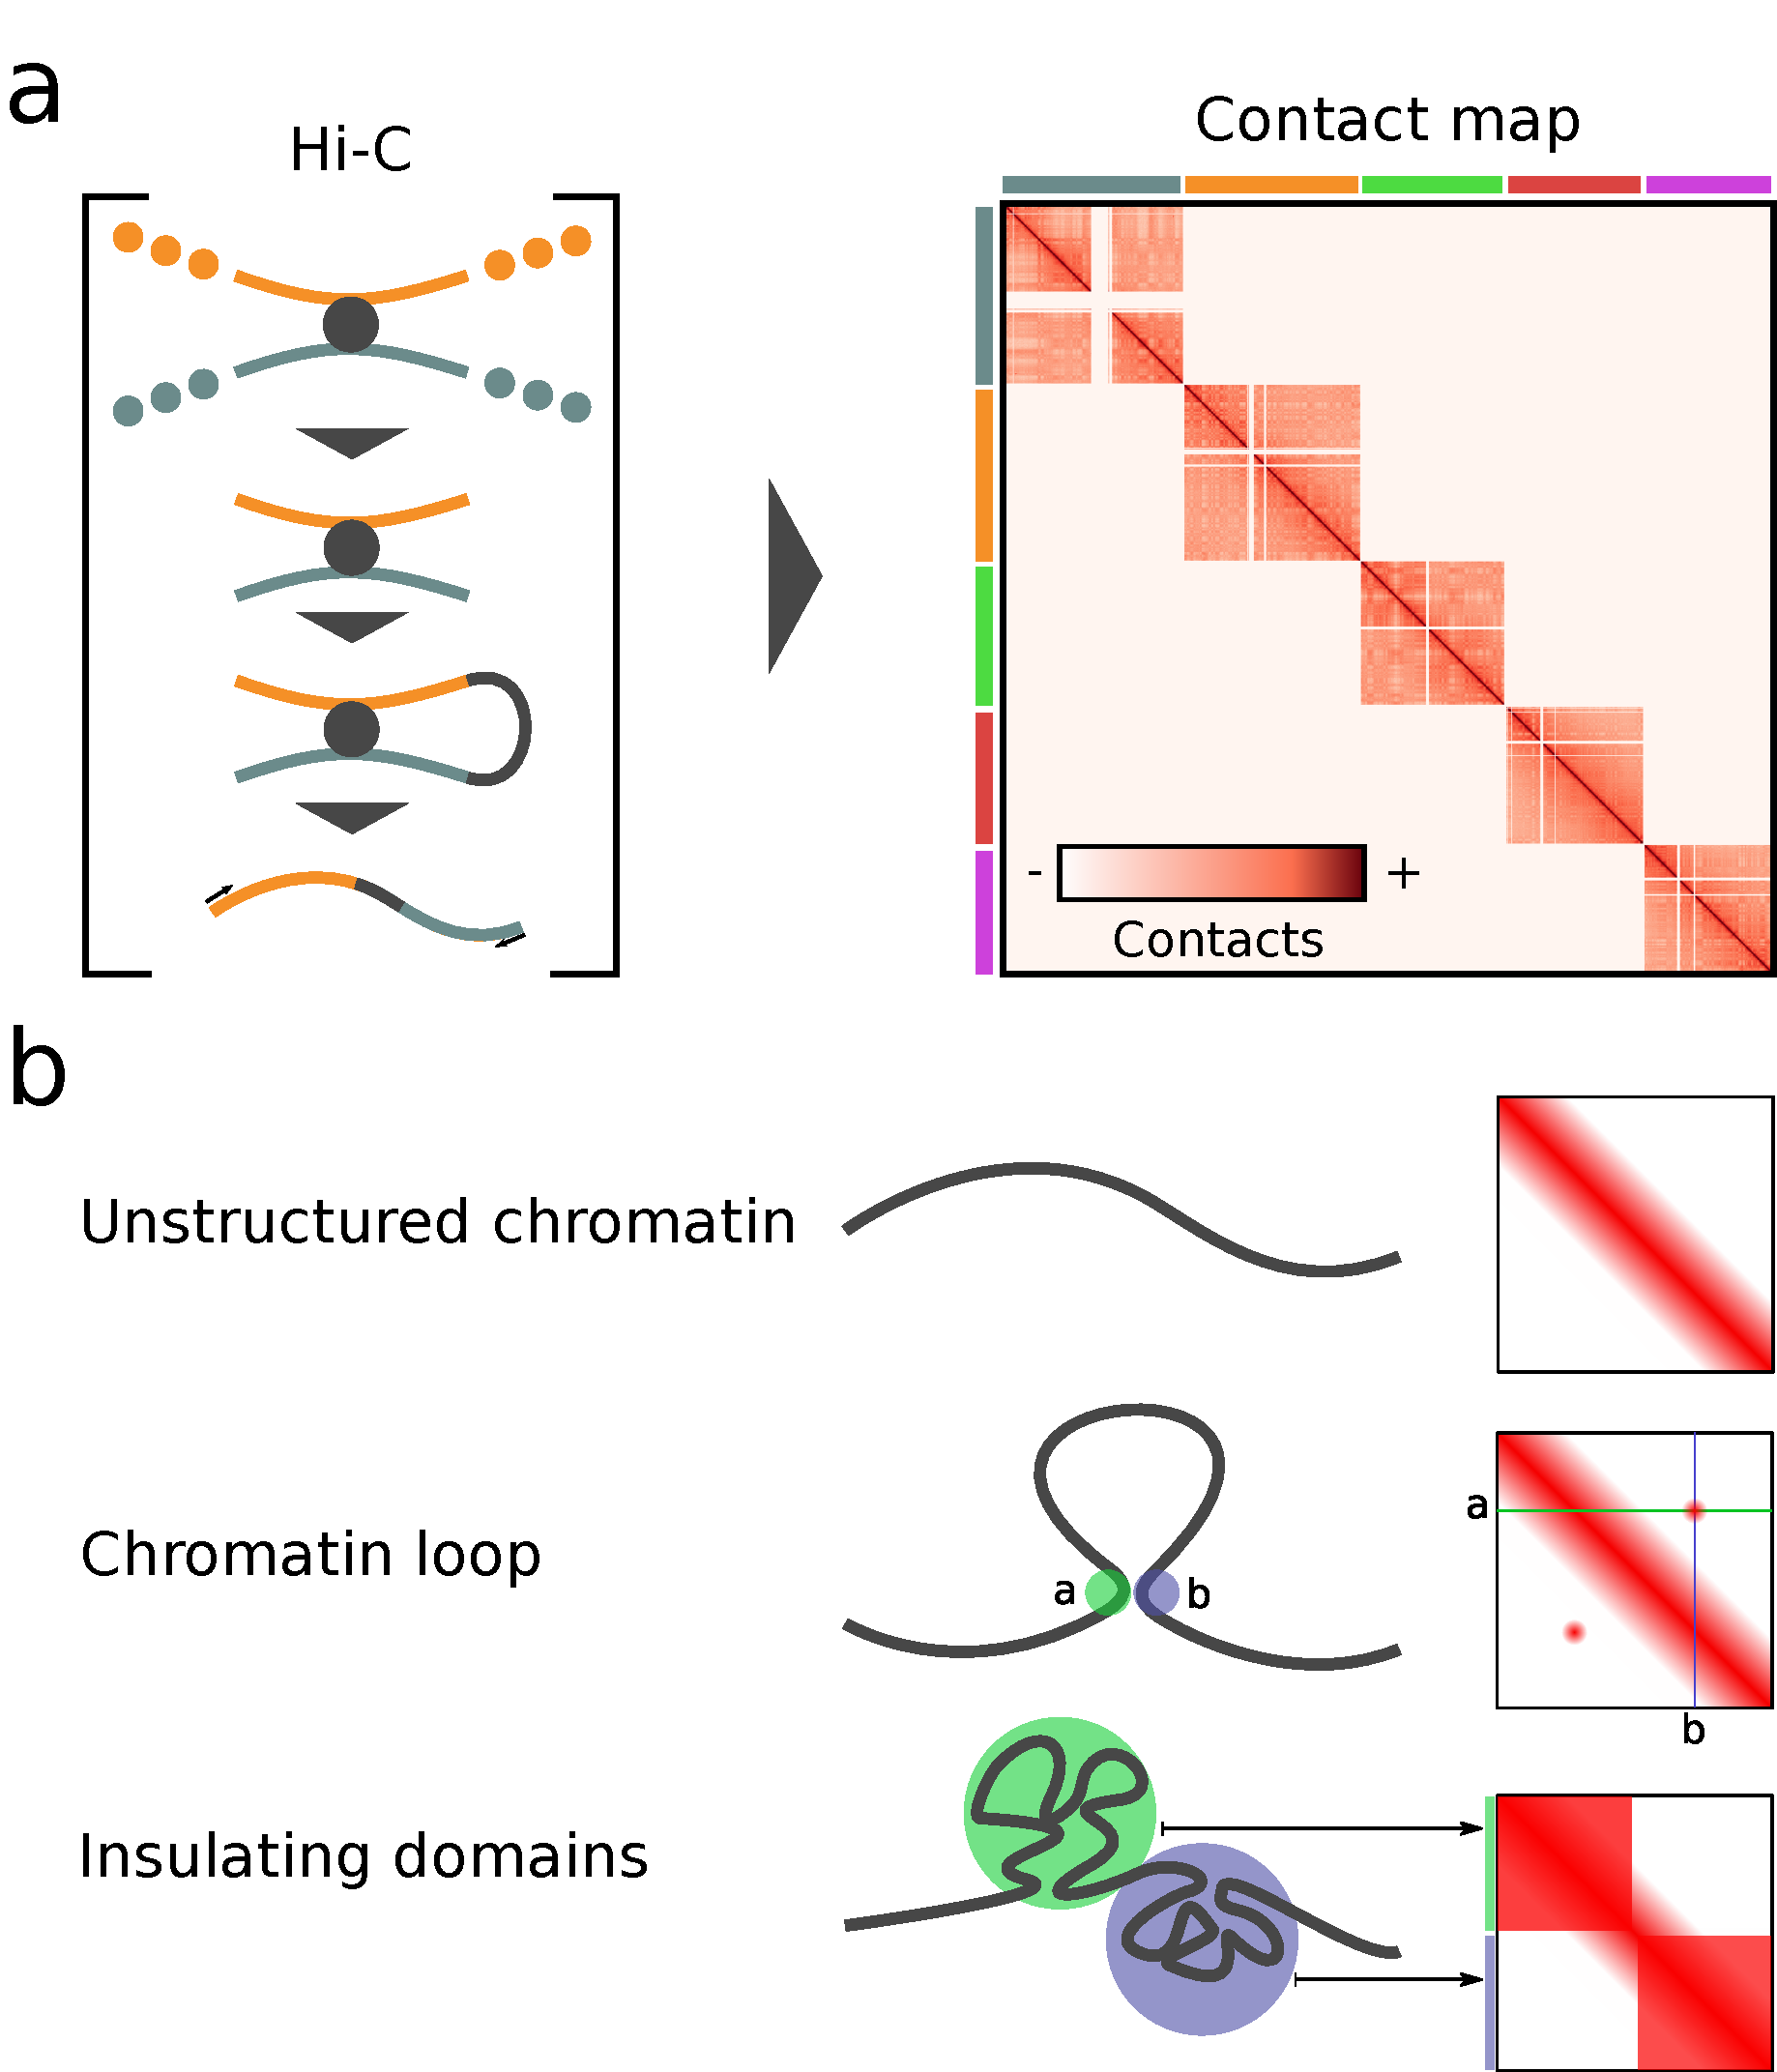
\includegraphics[width=\textwidth]{Parts/Part01/gfx/hic_interpretation.pdf}
    \caption{Interpretation of Hi-C contact maps: \textbf{a}: The Hi-C protocol (left) generates millions of read pairs representing contacts between genomic loci in a population of cells. Those contacts can be stored into an all-versus-all contact matrix (right) averaging all contacts in the population. Each chromosome in the matrix forms a square of strong self-interactions along the diagonal due to chromosomal territories. \textbf{b:} Within each chromosomal map, different contact patterns reflect specific conformations (right). The main feature of a contact map is the diagonal gradient (top) caused by the contact decay according to genomic distances. Chromatin loops between two anchor loci are visible as dots away from the diagonal (middle). Insulation domains form squares along the diagonal of a chromosome where loci within the same domain interact strongly, but interactions between domains are depleted}
	\label{fig:01-02:hic}
\end{figure}

In many eukaryotes, chromatin is also segregated into active and inactive compartments, commonly known as "euchromatin" and "heterochromatin" or A/B compartments. The A (active) compartment has higher GC content, gene density and gene expression than its counterpart \cite{lieberman-aidenComprehensiveMappingLongRange2009a}. A and B compartments also occupy separate spaces in the nucleus, whereas the A compartment is located towards the middle of the nucleus, the B compartment is relegated to the nuclear periphery and associated with lamina domains \cite{steenselLaminaAssociatedDomainsLinks2017}. This spatial segregation results in preferential physical interactions within the same compartment, which are reflected on Hi-C contact maps by a plaid-like pattern. 

\subsection{Analysis of chromosome contact maps}

The most visible element on any chromosome contact map is the diagonal gradient reflecting the power-law relationship between genomic distance and contact frequency. This is often called the distance-decay function or $P(s)$ where $s$ means genomic distance and $P$ probability of contacts. The slope of the $P(s)$ in itself holds information on the relative contribution of short range and long range contacts in the chromosome, which is linked to chromosome compaction.

Due to the high intensity of this gradient, other patterns of biological relevance are often obscured on the contact map. A common preprocessing step to account for it is to apply an \acrfull{o/e} normalization of the Hi-C map, where each pixel is divided by the average of its diagonal (Fig. \ref{fig:01-02:compartments}a). Lower intensity patterns such as domains, compartments and chromatin loop are easier to perceive on the resulting map.

After \acrshort{o/e} normalization, the compartment signal is generally the most salient feature on the contact maps. It can be extracted using \acrfull{PCA} on the normalized contact map \cite{lajoieHitchhikerGuideHiC2015} and retrieving the first few eigenvectors (i.e. principal component) explaining the most variance (Fig. \ref{fig:01-02:compartments}b). In some cases where compartment signal is weak (e.g. noisy datasets), the compartment signal may not be contained in the first eigenvector. A robust approach is to select the eigenvector with the strongest absolute correlation to an external signal known to be associated with active chromatin, such as gene expression or GC content \cite{sergeyvenevOpen2cCooltoolsV02021} (Fig. \ref{fig:01-02:compartments}c). The sign of the eigenvector is arbitrary, and it must be "phased" with the feature by flipping its sign to ensure a positive correlation with the said feature. In the phased vector, regions in the A compartment will contain positive values and \textit{vice versa}. The positions at which the sign changes are boundaries between different compartments (Fig. \ref{fig:01-02:compartments}d).

\begin{figure}[htb]
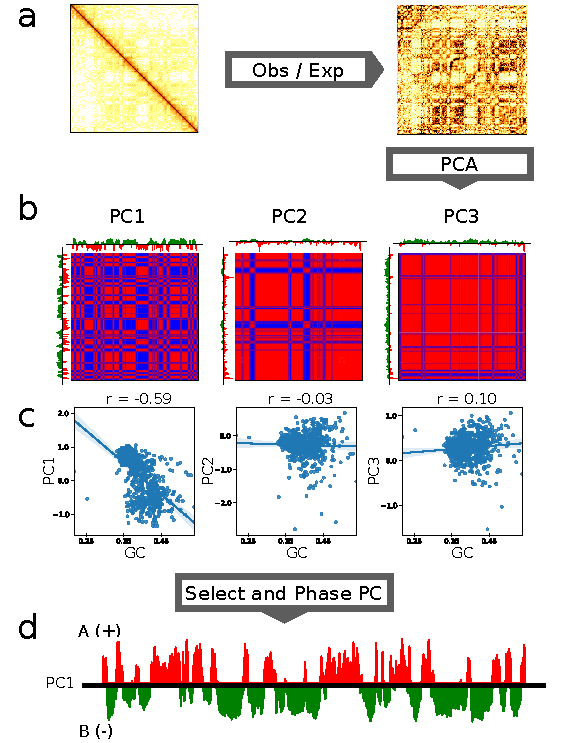
\includegraphics[width=0.95\textwidth]{Parts/Part01/gfx/hic_pca_compartments.pdf}
\caption{Representation and analysis of chromatin compartments in Hi-C. \textbf{a:} \acrfull{o/e} normalization is applied to the balanced contact map to remove the distance-decay gradient. Higher frequency of interactions within the same compartment result in a plaid-like pattern on chromosome contact maps. \textbf{b:} PCA is applied to the \acrshort{o/e} normalized contact map and the first few principal coponents (PC) are retained. For visualization, each PC is shown alongside with its outer, yielding the rank-1 reconstruction of the contact map. The outer product matrix is binarized (negative=blue, positive=red) to show the compartmentalization. \textbf{c:} The correlation of each PC with GC content is computed, to select the PC with the highest absolute correlation. \textbf{d:} The sign of PCs being meaningless, the selected PC is phased (by changing its sign in case of negative correlation) to ensure positive values represent A compartment.}
\label{fig:01-02:compartments}
\end{figure}

Another other useful vector often extracted from contact maps is the insulation score. As mentioned previously, many genomes are segmented into \acrshort{TAD}s containing frequently interacting regions, and often co-regulated genes. Regions in different \acrshort{TAD}s are insulated from each other, and the strength of this insulation can be measured at any given region as the ration of contacts across that region (upstream with downstream), relative to background on each side. Various derivatives of the insulation score have been developed and are used to detect \acrshort{TAD}s in several tools.

Some tools detect chromatin loops by looking for local enrichment of contacts, appearing as dots away from the diagonal. However, current loop detection algorithms suffer from low detection rates (recall). As such, an alternative approach is to focus on a set of genomic intervals of interest (e.g. binding sites of a transcription factor) and compute a window average of all pairs of intervals. The resulting average, often called pileup, can be used to visualize the present of chromatin loops between regions, or be compared between conditions.

In many cases, such cellular differentiation, it is useful to measure changes in Hi-C contacts between conditions. In that regard, the most global comparison, is to compute a similarity metric between pairs of samples. This is also useful as quality control, to compare technical (replicates) and biological (conditions) variability. The most commonly used methods do this using a metric based on the Pearson coefficient.

Rather than computing a single metric for each sample, an important application of Hi-C is to identify regions where the chromatin behaviour changes. Several methods aiming to achieve this are based on existing methods for RNA-seq. In this analogy, they consider each bin of the genome as a "gene" and their contacts as an expression count. They then model the bin intensity changes to identify those whose values is consistently changing between conditions across multiple replicates. This approach relies on solid statistical grounds, but it often does not address the question at hand. Often times, when analysing Hi-C data, we are interested in finding specific structures appearing or disappearing rather than a simple contact change at a region. The development of methods to discover relevant changes in chromatin conformmation is still an active area of research.

\section{Combining layers of biological informations}

The central dogma of biology - "DNA makes RNA and RNA makes protein" - exposes a linear set of reactions carrying the flow of information in living organisms. It is now known that these reactions by themselves are hardly sufficient to explain the complexity of biological processes. The fine tuning required for proper regulation is achieved through feedback loops and cross-talk between the different types of molecules (Fig. \ref{fig:01-02:central-dogma}). Common examples are methylation of DNA by proteins to reduce gene expression \cite{zemachGenomeWideEvolutionaryAnalysis2010}, noncoding RNAs recruiting proteins to repress transcription \cite{wangLongNoncodingRNA2018} or directly repressing translation by preventing ribosome binding \citep{sharmaSmallRNARegulates2007,vecerekControlFurSynthesis2007}.

\begin{figure}[htb]
    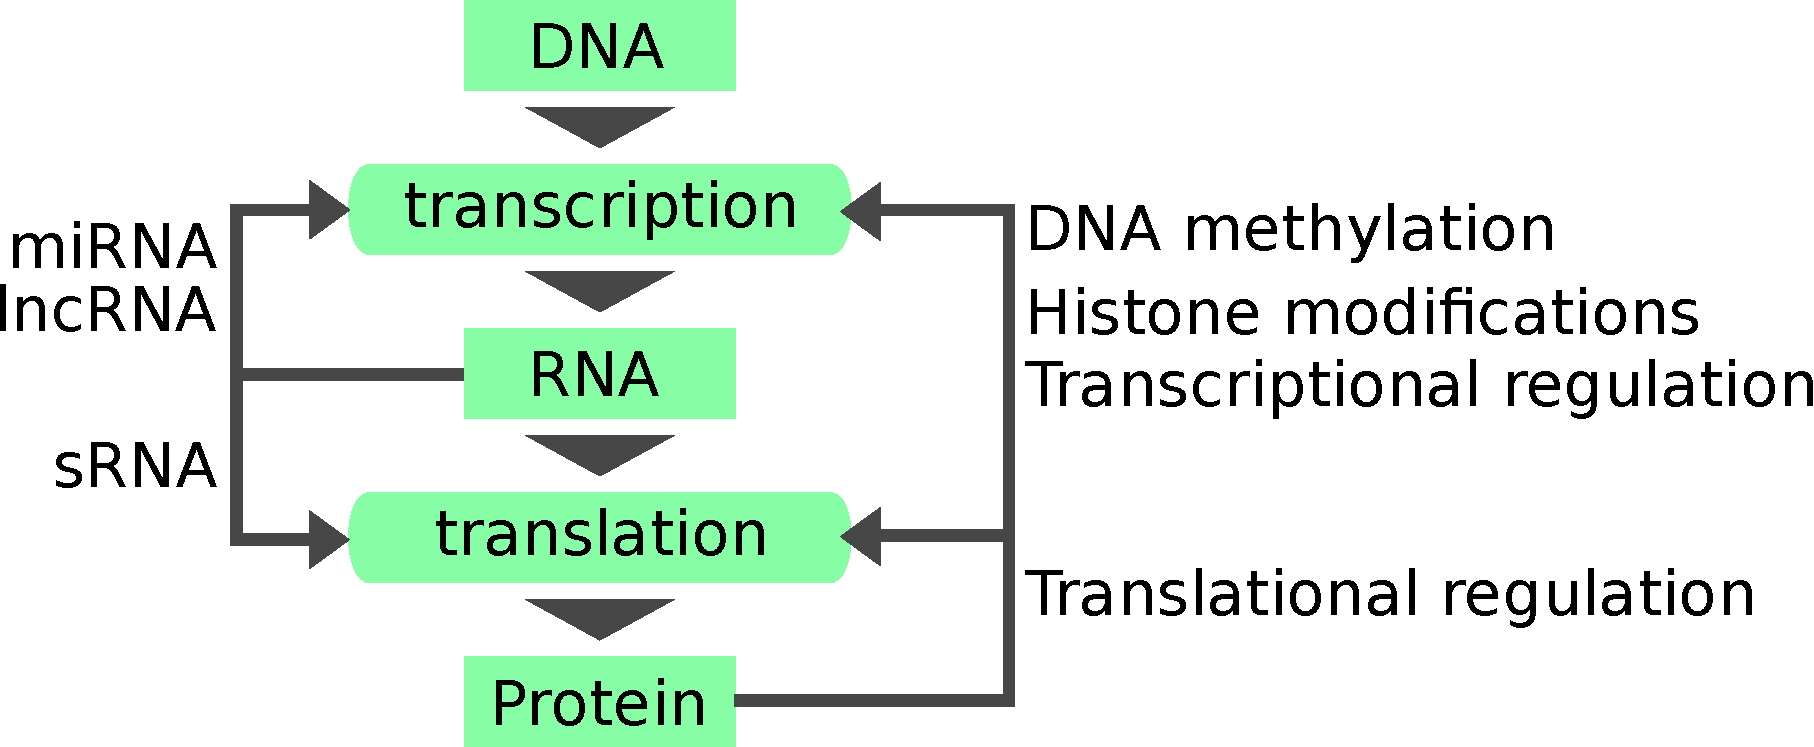
\includegraphics[width=0.8\textwidth]{Parts/Part01/gfx/central_dogma_regulation.pdf}
    \caption{Central dogma of molecular biology. Products and reactions from the central dogma are shown in green, with grey arrows showing some of the regulatory interactions between the different biomolecules.}
    \label{fig:01-02:central-dogma}
\end{figure}

There is now a growing area of research focusing on the development of methods that combine these layers of information. They aim to gain an integrative view of biology to better model the behaviour of molecular networks. This is done by combining "omics" datasets measuring various biomolecules, such as genetic mutations, gene expression, protein binding, histone modifications or protein abundance.

One of the main challenges is to find efficient ways to combine these informations to extract meaningful biological information. More often than not, they are analysed separately to find regions of deregulation common to the different layers. But there have already been attempts at fully integrating these levels of informations %MOFA, DL from Anshul Kundaje

Another challenge is the difficulty to combine different datasets due to technical heterogeneities or biological differences such as different strains or experimental conditions.
